% Current method: user-confirmed F32, Tong hop last row 18 (2026-10-18).
% F24 historical hashes do not identify this F32 revision. See support/F32_REVISION_EVIDENCE.md.
% Paper name Strata-BEV14 maps to the unchanged hist14 v1 checkpoint encoding.

MobilePIXORNeXt maps a LiDAR scan to class-labelled oriented BEV boxes through deterministic feature encoding, a compact convolutional hierarchy, multiscale fusion, and grouped prediction heads. Figure~\ref{fig:r37_overview} summarizes the configuration used as the main detector, denoted R37-F32 here to distinguish it from the earlier F24 run. Its outputs describe horizontal location, footprint dimensions, orientation, and localization quality. Vertical box coordinates are not predicted by this configuration; any separately trained 3D extension is evaluated as a distinct variant.

\begin{figure*}[t]
    \centering
    \paperfigure{pipeline_overview.pdf}{30mm}{Source: slide PDF page 1; complete overview page, preserving vector labels and embedded point-cloud images.}
    \caption{Overview of MobilePIXORNeXt. Strata-BEV14 converts the scan into a fixed statistical grid; the detector predicts class heatmaps, center offsets, footprint dimensions, doubled yaw, and localization quality. The main model predicts oriented BEV footprints, shown over the 3D input cloud. The dashed feedback path is used only in training. FL denotes Gaussian focal classification, BCE supervises localization quality, and T-SBUW denotes the adaptive task balancing described in the text.}
    \label{fig:r37_overview}
\end{figure*}


\subsection{Strata-BEV14 point-cloud encoding}
\label{sec:rich_bev14}

The representation is inspired by the height-stratified BEV design of TriBand-BEV~\cite{khoshkdahan2026triband}, whose three channels store band-wise maximum corrected reflectance. We retain the idea of summarizing vertical structure on a horizontal grid, but use different band definitions and statistical channels. We call the two configurations Strata-BEV8 and Strata-BEV14; their suffixes denote channel counts, not height-band counts. These names describe our configured encodings, rather than a reproduction of TriBand-BEV.

Height histograms provide another source of inspiration~\cite{zhou2025pillarhist}. We use four log-scaled count bins, cell statistics, and mean subcell offsets. The resulting fourteen-channel raster is deterministic; it does not reproduce the learned pillar encoder in that work or establish its reported quantization benefits for our detector.

A scan is represented by $\mathcal P=\{(x_i,y_i,z_i,\iota_i)\}_{i=1}^{N_{\mathrm{pts}}}$, where $\iota_i$ is reflectance. The LiDAR frame uses forward $x$, leftward $y$, and upward $z$. We retain finite points within the region $[0,70.4]\times[-40,40]\times[-2.5,1.0]$~m, applying strict bounds with a $0.001$~m inward margin. A horizontal resolution of $\Delta_x=\Delta_y=0.1$~m produces $800\times704$ cells. Point assignment uses
\begin{equation}
    u_{\mathrm{in}}=\left\lfloor\frac{x_i-x_{\min}}{\Delta_x}\right\rfloor,
    \qquad
    v_{\mathrm{in}}=\left\lfloor\frac{y_i-y_{\min}}{\Delta_y}\right\rfloor.
    \label{eq:input_grid}
\end{equation}

Strata-BEV14 encodes each occupied cell using the fourteen statistics in Table~\ref{tab:rich_bev14}. Heights are normalized as $\zeta_i=(z_i-z_{\min})/(z_{\max}-z_{\min})$, and reflectance is clipped to $[0,1]$. Four equal-height intervals summarize the vertical distribution. Their count channels and the total-density channel use
\begin{equation}
    d_{\log}(N)=\min\left(1,\frac{\log(1+N)}{\log(33)}\right),
    \label{eq:density_encoding}
\end{equation}
where $N$ is the corresponding cell or bin count. These channels are density statistics rather than histogram probabilities. The remaining statistics describe height variation, reflectance, occupancy, and subcell point locations. Empty cells are zero, and the resulting input is $\mathbf X\in\mathbb R^{B\times14\times800\times704}$.

\begin{table}[t]
    \caption{Strata-BEV14 channels, indexed from zero. All statistics are computed over points in one input cell.}
    \label{tab:rich_bev14}
    \centering\small
    \begin{tabular}{@{}p{0.15\columnwidth}p{0.77\columnwidth}@{}}
        \toprule
        Channels & Cell statistics \\
        \midrule
        0--3 & Log-normalized counts in four equal-height intervals. \\
        4--7 & Maximum, mean, span, and population standard deviation of $\zeta_i$. \\
        8--9 & Maximum and mean clipped reflectance. \\
        10--11 & Log-normalized total count and binary occupancy. \\
        12--13 & Mean point displacement from the input-cell center, divided by $\Delta_x$ or $\Delta_y$ and clipped to $[-0.5,0.5]$. \\
        \bottomrule
    \end{tabular}
\end{table}

This deterministic encoding retains vertical summaries while allowing the learned network to operate entirely on a horizontal grid. The normalized point displacements describe the distribution of observations within an input cell; they are distinct from the metric object-center offsets predicted by the detector.

Strata-BEV8 starts with three occupancy channels for equal-height bands. These are followed by maximum and mean normalized height, maximum and mean clipped reflectance, and total log-density. Its occupancy bands indicate whether a return exists; they do not store band-wise reflectance. Strata-BEV14 changes the vertical summary to four log-count bands and adds height span, height standard deviation, whole-cell occupancy and mean subcell offsets. Consequently, the eight-channel encoding is not simply a subset of the fourteen-channel tensor. Both use the configured sensor-frame height interval; neither applies TriBand-BEV's ground-referenced band thresholds or reflectance offset and gain. The implementation keys remain \texttt{rich8} and \texttt{hist14} (v1) for reproducibility.

\subsection{Compact convolutional hierarchy}
\label{sec:method_backbone}

The stem contains two $3\times3$ convolutions with 32 output channels and strides two and one, respectively. Each is followed by batch normalization (BN) and SiLU. Three subsequent stages begin with a stride-two $3\times3$ convolution and contain 3, 4, and 2 residual blocks. Their outputs have 48, 96, and 128 channels at strides 4, 8, and 16. We index features by their spatial stride, $\mathbf F^{(r)}$, to make the resolution of each connection explicit.

Figure~\ref{fig:backbone} specifies the feature hierarchy and shared grouped heads. The final fusion width is 32 channels; it should not be confused with the earlier F24 configuration carrying the same workbook identifier.

\begin{figure*}[t]
    \centering
    \paperfigure{backbone_f32.pdf}{44mm}{Source: current slide PDF page 3; residual block on page 4 and fusion on page 5.}
    \caption{Final backbone, fusion neck, and prediction heads. Spatial strides are 2 at the stem and 4, 8, and 16 at the three subsequent stages. Lateral widths are 32, 48, and 48, and the final shared feature has shape $32\times200\times176$. Prediction maps have 176 columns; the Pedestrian/Cyclist heatmap has two channels. Stages are identified here by strides 4/8/16; the drawing retains legacy C2/C3/C4 labels, and its deepest stage label refers to the stride-16 stage. Each group uses a shared $3\times3$--BN--SiLU stem; each private Conv box abbreviates $3\times3$--BN--SiLU followed by a $1\times1$ output projection.}
    \label{fig:backbone}
\end{figure*}

The residual block adopts large-kernel depthwise spatial mixing and inverted channel expansion, following modern convolutional design principles~\cite{liu2022convnext}. For a $C$-channel input $\mathbf Z$, its transformation is
\begin{align}
    \mathbf V &= \operatorname{BN}(\operatorname{DWConv}_{7\times7}(\mathbf Z)),\nonumber\\
    \mathbf R &= \operatorname{BN}\!\left(W_{\mathrm{red}}\,
        \operatorname{SiLU}(W_{\mathrm{exp}}\mathbf V)\right),\nonumber\\
    \mathbf Z' &= \mathbf Z+\boldsymbol\gamma_{\mathrm{blk}}\odot\mathcal S(\mathbf R).
    \label{eq:next_block}
\end{align}
Here $W_{\mathrm{exp}}$ and $W_{\mathrm{red}}$ are $1\times1$ convolutions that expand channels from $C$ to $2.5C$ and project them back to $C$. The operator $\mathcal S$ denotes block-level SimAM, defined below. The learned channel-wise residual scale $\boldsymbol\gamma_{\mathrm{blk}}$ is initialized to $10^{-5}$. The final model uses ordinary depthwise convolutions without structural reparameterization or an additional detail branch.

\subsection{Block-level SimAM refinement}
\label{sec:method_refinement}

The final model applies SimAM~\cite{yang2021simam} inside every residual block of the three backbone stages, corresponding to C3, C4, and C5 at strides 4, 8, and 16. With stage depths $(3,4,2)$, the backbone contains nine SimAM operators. Each operator acts on $\mathbf R$, the output of the channel-reduction convolution and its BN, before the existing LayerScale and shortcut addition in Eq.~\ref{eq:next_block}. Figure~\ref{fig:r37_refinement} shows this ordering. Thus, attention changes the residual update while leaving the identity shortcut intact.

For a residual tensor $\mathbf R\in\mathbb R^{B\times C\times H\times W}$, let $\mu_c^{\mathrm{sp}}$ be the spatial mean within channel $c$ and define
\begin{equation}
    \nu_c^{\mathrm{sp}}=\frac{\sum_{v,u}(R_{cvu}-\mu_c^{\mathrm{sp}})^2}{\max(HW-1,1)}.
    \label{eq:simam_variance}
\end{equation}
The batch index is omitted; statistics are computed independently for each example and channel. The elementwise gate and attended update are
\begin{align}
    A_{cvu} &= \sigma\!\left(
        \frac{(R_{cvu}-\mu_c^{\mathrm{sp}})^2}
        {4(\nu_c^{\mathrm{sp}}+\lambda_{\mathrm{sim}})}+\frac12\right),\nonumber\\
    \mathcal S(\mathbf R) &= \mathbf A\odot\mathbf R,
    \label{eq:block_simam}
\end{align}
with $\lambda_{\mathrm{sim}}=10^{-4}$. The gate assigns larger weights to activations whose squared deviation from the channel mean is larger relative to its spatial variance. This operation uses feature statistics rather than point occupancy or learned query--key interactions. Spatial moments and gate values are computed in FP32, then the gate is cast to the feature dtype for multiplication.

SimAM introduces no learned parameters in this placement. The existing channel-wise scale $\boldsymbol\gamma_{\mathrm{blk}}$ controls the attended residual; there is no additional scalar wrapper. This differs from applying a residual attention adapter after an entire stage. The final model enables block attention at all three stages, with no separate stage-level attention or focal-context module.

\begin{figure*}[t]
    \centering
    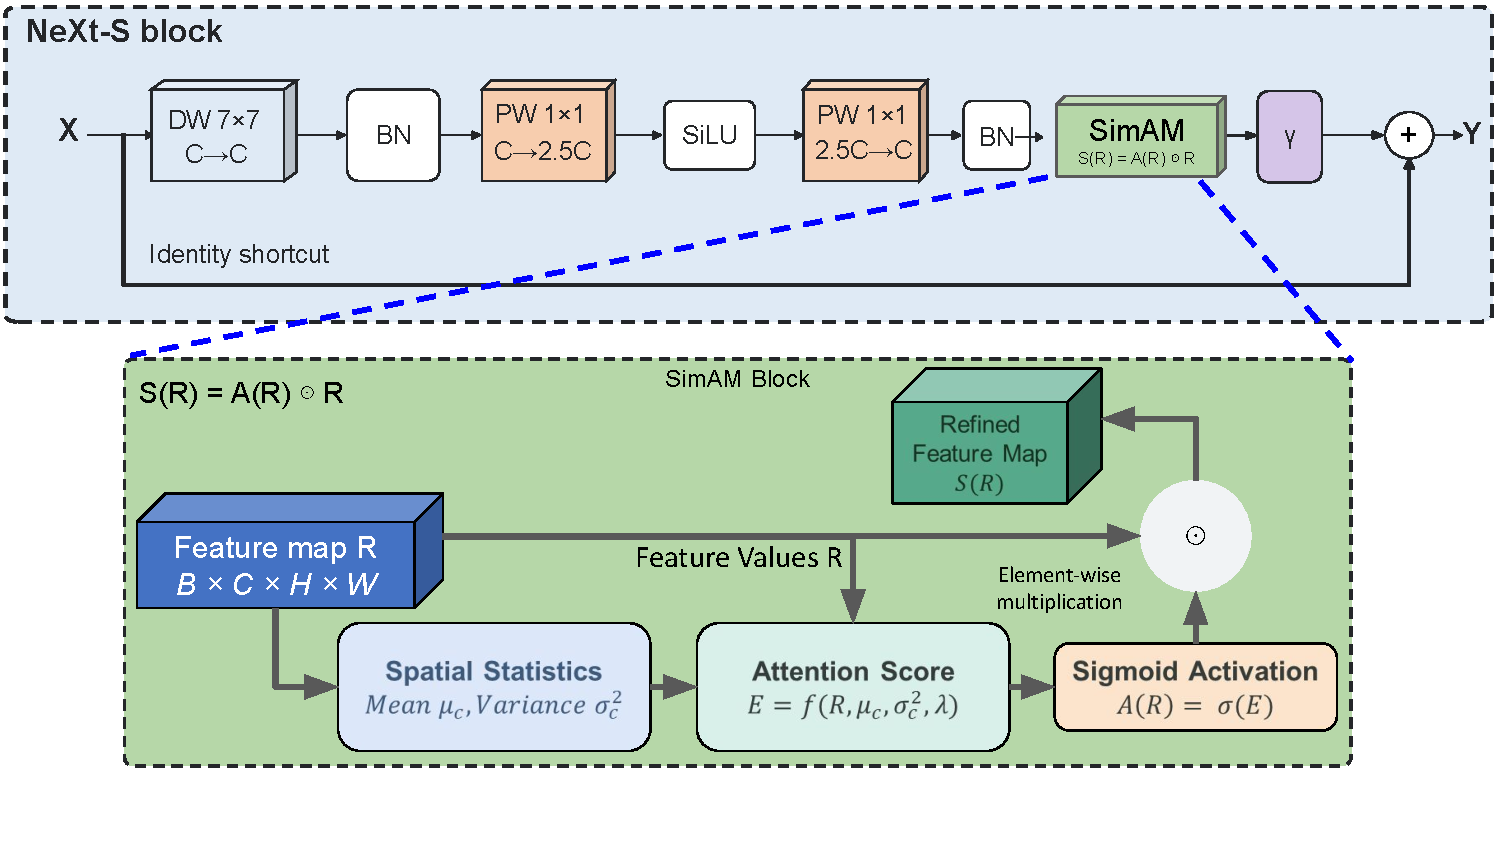
\includegraphics[width=\textwidth]{figures/next_simam_block.pdf}\\[6pt]
    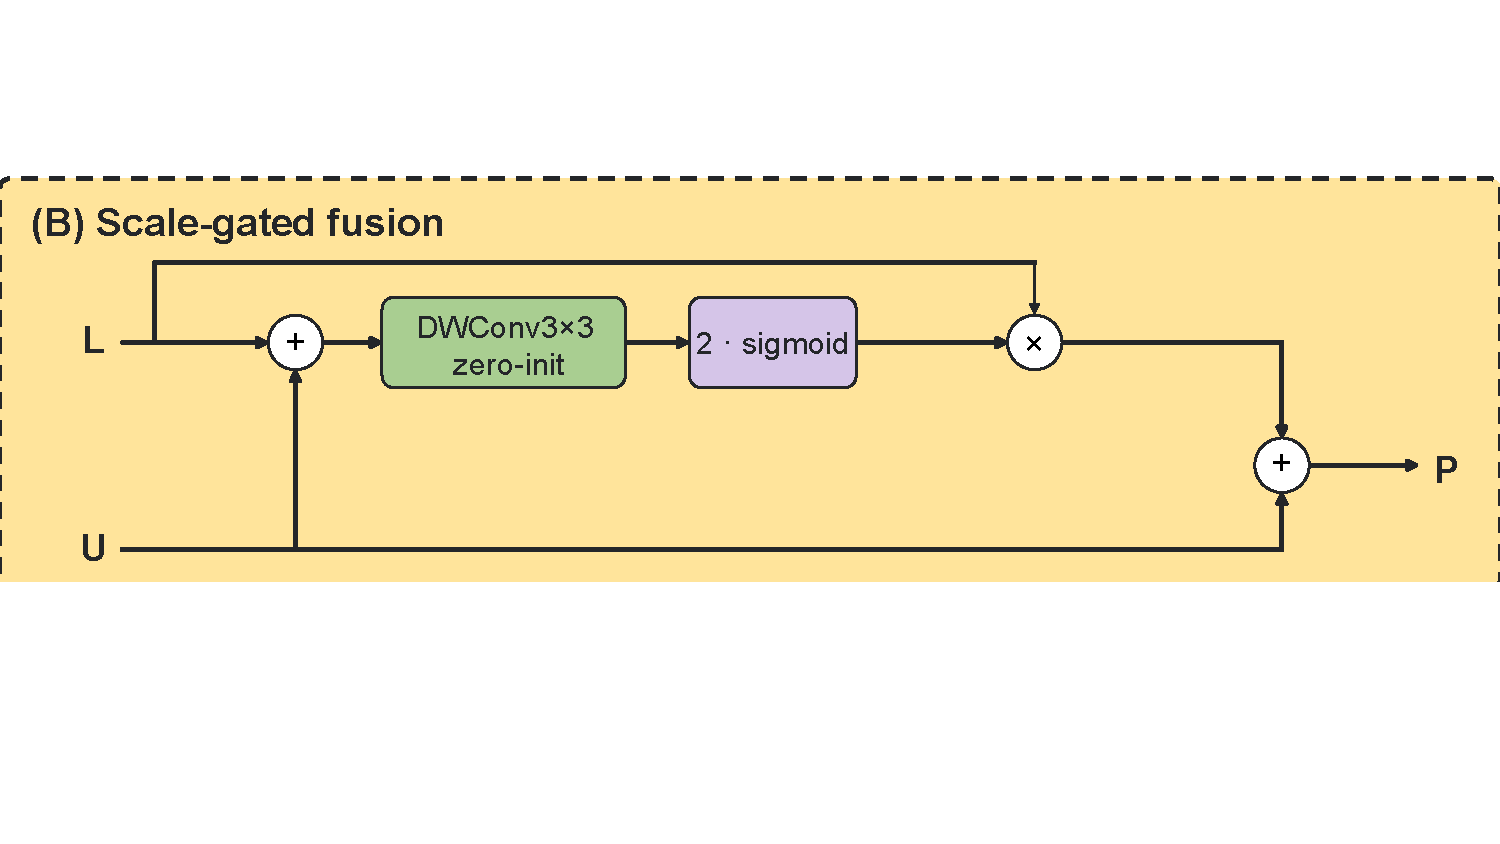
\includegraphics[width=0.70\textwidth]{figures/scale_gated_fusion.pdf}
    \caption{Two building blocks extracted as vector graphics from the authors' slide export. (A) NeXt residual block with SimAM after projection BN and before LayerScale. The SimAM operator acts on the intermediate residual tensor $\mathbf R$ in Eq.~\ref{eq:next_block}, consistently labeled R in the drawing. (B) Scale-gated fusion of lateral feature $\mathbf L$ and top-down feature $\mathbf U$, yielding $\mathbf P$. Addition and elementwise multiplication are shown explicitly.}
    \label{fig:r37_refinement}
\end{figure*}


\subsection{Scale-gated multiscale fusion}
\label{sec:method_neck}

The neck projects the stride-16 and stride-8 features to 48 channels, and the stride-4 feature to 32 channels. At stride eight, bilinear upsampling of the deepest lateral feature is followed by a depthwise $3\times3$ convolution, BN, and SiLU. The resulting top-down feature $\mathbf U_8$ is fused with lateral feature $\mathbf L_8$. A second bilinear upsampling and a standard $3\times3$ projection from 48 to 32 channels produce $\mathbf U_4$ for fusion with $\mathbf L_4$. Interpolation uses \texttt{align\_corners=False}.

Figure~\ref{fig:r37_refinement}(B) illustrates the fusion operator. At each fusion stride $r\in\{4,8\}$,
\begin{align}
    \mathbf G_r &= 2\sigma\!\left(
        \operatorname{DWConv}_{3\times3,r}(\mathbf L_r+\mathbf U_r)\right),\nonumber\\
    \mathbf P^{(r)} &= \mathbf U_r+\mathbf G_r\odot\mathbf L_r.
    \label{eq:scale_gated_fusion}
\end{align}
Gate weights and biases are zero-initialized, so fusion initially reduces to addition. A final $3\times3$ convolution from 32 to 32 channels, BN, and SiLU produce the shared detector feature $\mathbf F_{\mathrm{out}}\in\mathbb R^{B\times32\times200\times176}$. The gate can adjust each lateral response using information from both paths without replacing the top-down feature.

\subsection{Grouped prediction and target assignment}
\label{sec:method_heads}

The first task group contains Car ($K_1=1$), and the second contains Pedestrian and Cyclist ($K_2=2$). Each group first applies a shared $3\times3$ convolution with 32 channels, BN, and SiLU. Its output feeds five branches for classification, center offset, log-size, doubled yaw, and quality. Each branch contains one private $3\times3$ convolution with 32 channels, BN, and SiLU, followed by a $1\times1$ output convolution. Each prediction path therefore still traverses two $3\times3$ convolutions, while its first transformation is shared across tasks. The two groups own separate shared convolutions and branch weights. Geometry and quality maps are shared across the classes within a group.

For a group with $K_g$ classes, the output channel counts are $(K_g,2,2,2,1)$. At output location $(u,v)$, the geometric targets are
\begin{align}
    \mathbf o^* &= \begin{pmatrix}
        x^*-x_{\min}-u s_{\mathrm{out}}\Delta_x\\
        y^*-y_{\min}-v s_{\mathrm{out}}\Delta_y
    \end{pmatrix},\nonumber\\
    \mathbf d^* &= (\log w^*,\log l^*),\qquad
    \mathbf a^*=(\cos2\psi^*,\sin2\psi^*),
    \label{eq:regression_targets}
\end{align}
where $s_{\mathrm{out}}=4$ and sizes inside logarithms are expressed numerically in metres. The doubled angle represents footprint orientation modulo $\pi$.

Classification uses class-specific Gaussian heatmaps with peaks at quantized object centers. The radius is determined from the footprint dimensions in output cells using overlap setting 0.1 and a minimum radius of four cells. Regression supervision occupies a disk with half that heatmap radius. Where disks overlap, cells are assigned to the nearest continuous object center, with quantized center cells reserved for their owning targets. This produces a single valid regression target per group and location, indicated by $\mathbf M_{\mathrm{reg}}$.

\subsection{Oriented geometry and quality supervision}
\label{sec:method_objective}

The OGA objective combines classification, coordinate regression, footprint geometry, and quality prediction. Classification uses the Gaussian focal form: unit-valued heatmap peaks have modulating factor $(1-p_{\mathrm{cls}})^2$, while other cells use $p_{\mathrm{cls}}^2(1-Y^*)^4$. The summed loss is normalized by the number of positive peaks; an image batch without peaks retains the negative sum. Offset, log-size, and doubled-yaw losses use Smooth-L1 with transition parameter one, averaged over the valid regression elements. Numerical normalization adds $10^{-4}$ to the element count.

For each valid regression cell, predicted and target footprints are decoded into four corners. Following Marginalized Generalized Intersection over Union (MGIoU)~\cite{le2026mgiou}, both rectangles are projected onto the length and width axes of the prediction and target. On each axis, we compute one-dimensional Generalized Intersection over Union (GIoU)~\cite{rezatofighi2019giou}. For projection axis $k$, let $I_k$, $U_k$, and $E_k$ be the intersection, union, and enclosing interval lengths. Define
\begin{align}
    g_k &= \frac{I_k}{U_k}-\frac{E_k-U_k}{E_k},\nonumber\\
    \bar g &= \frac14\sum_{k=1}^{4}g_k,\qquad
    \ell_{\mathrm{proj}}=\frac{1-\bar g}{2}.
    \label{eq:projected_geometry}
\end{align}
Here $\bar g$ is the rectangle-specific MGIoU similarity and $\ell_{\mathrm{proj}}$ is its normalized loss. Denominators are floored at $10^{-6}$. This compares one-dimensional projections rather than computing polygon intersection area.

The corner term measures average L1 corner discrepancy under two equivalent correspondences. Let $\widehat{\mathbf c}_m$ and $\mathbf c_m^*$ denote ordered footprint corners, and let $\Pi_\pi$ contain the identity and the permutation induced by a $\pi$ rotation. Then
\begin{equation}
    \ell_{\mathrm{corner}}=
    \frac{\displaystyle\min_{\pi\in\Pi_\pi}\frac14
        \sum_{m=1}^{4}\|\widehat{\mathbf c}_m-\mathbf c_{\pi(m)}^*\|_1}
    {\max\!\left(\sqrt{(w^*)^2+(l^*)^2},10^{-6}\right)}.
    \label{eq:symmetric_corners}
\end{equation}
Target-diagonal normalization scales the discrepancy relative to object size, and the two correspondences respect the doubled-angle representation. The geometry objective is the mean of $\ell_{\mathrm{proj}}+\beta_{\mathrm{corner}}\ell_{\mathrm{corner}}$ over valid cells, with $\beta_{\mathrm{corner}}=1$. Geometry calculations use FP32, clamp log-dimensions to $[-10,10]$, and use zero yaw when the doubled-angle vector norm is below $10^{-6}$.

The IQA branch predicts $\hat q=\sigma(\hat Z_{\mathrm{qual}})$ and is supervised at valid regression cells using binary cross-entropy. Its target is
\begin{equation}
    q_{\mathrm{proj}}^*=\operatorname{stopgrad}
        \bigl(\operatorname{clip}(\bar g,0,1)\bigr).
    \label{eq:quality_target}
\end{equation}
The target uses the clipped MGIoU similarity, not the geometry loss. It is detached from box decoding, so this supervision does not backpropagate through the target geometry. Although the implementation names the branch IoU-aware quality, the final model learns a projection-based similarity, not exact BEV or 3D IoU. Its coefficient before adaptive balancing is one.

\subsection{Adaptive task balancing}
\label{sec:method_balance}

Each group independently balances six loss terms, indexed by $\mathcal T=\{\mathrm{cls},\mathrm{off},\mathrm{size},\mathrm{yaw},\mathrm{geo},\mathrm{qual}\}$ with $J=6$. Learned logits $a_k$ determine positive weights through a bounded temperature softmax:
\begin{align}
    \bar a_k &= b_{\mathrm{uw}}\tanh(a_k/b_{\mathrm{uw}}),\nonumber\\
    \omega_k &= J\frac{\exp(\bar a_k/\tau_{\mathrm{uw}})}
        {\sum_{j\in\mathcal T}\exp(\bar a_j/\tau_{\mathrm{uw}})},
    \label{eq:task_weights}
\end{align}
where $b_{\mathrm{uw}}=3$ and $\tau_{\mathrm{uw}}=2$. Zero-initialized logits give unit initial weights. An exponential moving average $\mu_k$ tracks the detached, floored task loss with momentum $\beta_{\mathrm{EMA}}=0.99$, initialized from the first training batch. For group $g$, the balanced objective is
\begin{equation}
    \mathcal L_g=\left(\frac1J\sum_{k\in\mathcal T}\mu_k\right)
        \sum_{k\in\mathcal T}\omega_k
        \frac{\mathcal L_k}{\max(\mu_k,10^{-4})}.
    \label{eq:balanced_objective}
\end{equation}
The full loss is $\mathcal L_{\mathrm{total}}=0.5\mathcal L_1+0.5\mathcal L_2$. Running-scale normalization compensates for differences in task-loss magnitude before weighting. These adaptive weights are optimization variables, not calibrated estimates of statistical uncertainty. The two groups introduce twelve training-only logits, separate from the detector parameters used at inference.

\subsection{Decoding and inference}
\label{sec:method_decode}

Predicted offsets are in metres relative to output-grid origins. Box decoding is
\begin{align}
    \hat x &= x_{\min}+u s_{\mathrm{out}}\Delta_x+\hat o_x,\nonumber\\
    \hat y &= y_{\min}+v s_{\mathrm{out}}\Delta_y+\hat o_y,\nonumber\\
    \hat w &= \exp(\hat d_1),\qquad \hat l=\exp(\hat d_2),\nonumber\\
    \hat\psi &= \tfrac12\operatorname{atan2}(\hat a_2,\hat a_1).
    \label{eq:box_decode}
\end{align}
No half-cell shift is added. Classification and quality predictions are combined as
\begin{equation}
    s_{\mathrm{det}}=p_{\mathrm{cls}}^{1-\alpha_{\mathrm{score}}}
        \hat q^{\alpha_{\mathrm{score}}},\qquad \alpha_{\mathrm{score}}=0.5.
    \label{eq:quality_ranking}
\end{equation}
Candidates are selected from $3\times3$ local maxima of this ranking score independently for each class. Both $p_{\mathrm{cls}}$ and $s_{\mathrm{det}}$ must exceed 0.05. Classwise rotated BEV non-maximum suppression uses an IoU threshold of 0.1, followed by a global limit of 500 detections per scan. These decoding thresholds are separate from the overlap thresholds used to evaluate detection accuracy.

The complete F32 detector has 753,569 learned parameters, excluding the adaptive loss weights. The selected workbook configuration uses hybrid ground-truth sampling. Section~\ref{sec:experiments} distinguishes the verified model specification from training and timing settings still requiring the final run records.
